\documentclass{article}

\usepackage{graphicx}
\usepackage{tikz}
\usepackage{tikzsymbols}
\usetikzlibrary{calc,patterns,shapes.geometric}
\pagestyle{empty}
\usepackage[margin=0pt]{geometry}
\geometry{papersize={14in,12in}}

\def\centerarc[#1](#2)(#3:#4:#5){\draw[#1] ($(#2)+({#5*cos(#3)},{#5*sin(#3)})$) arc (#3:#4:#5);}

\begin{document}
	\begin{figure}
		\centering
		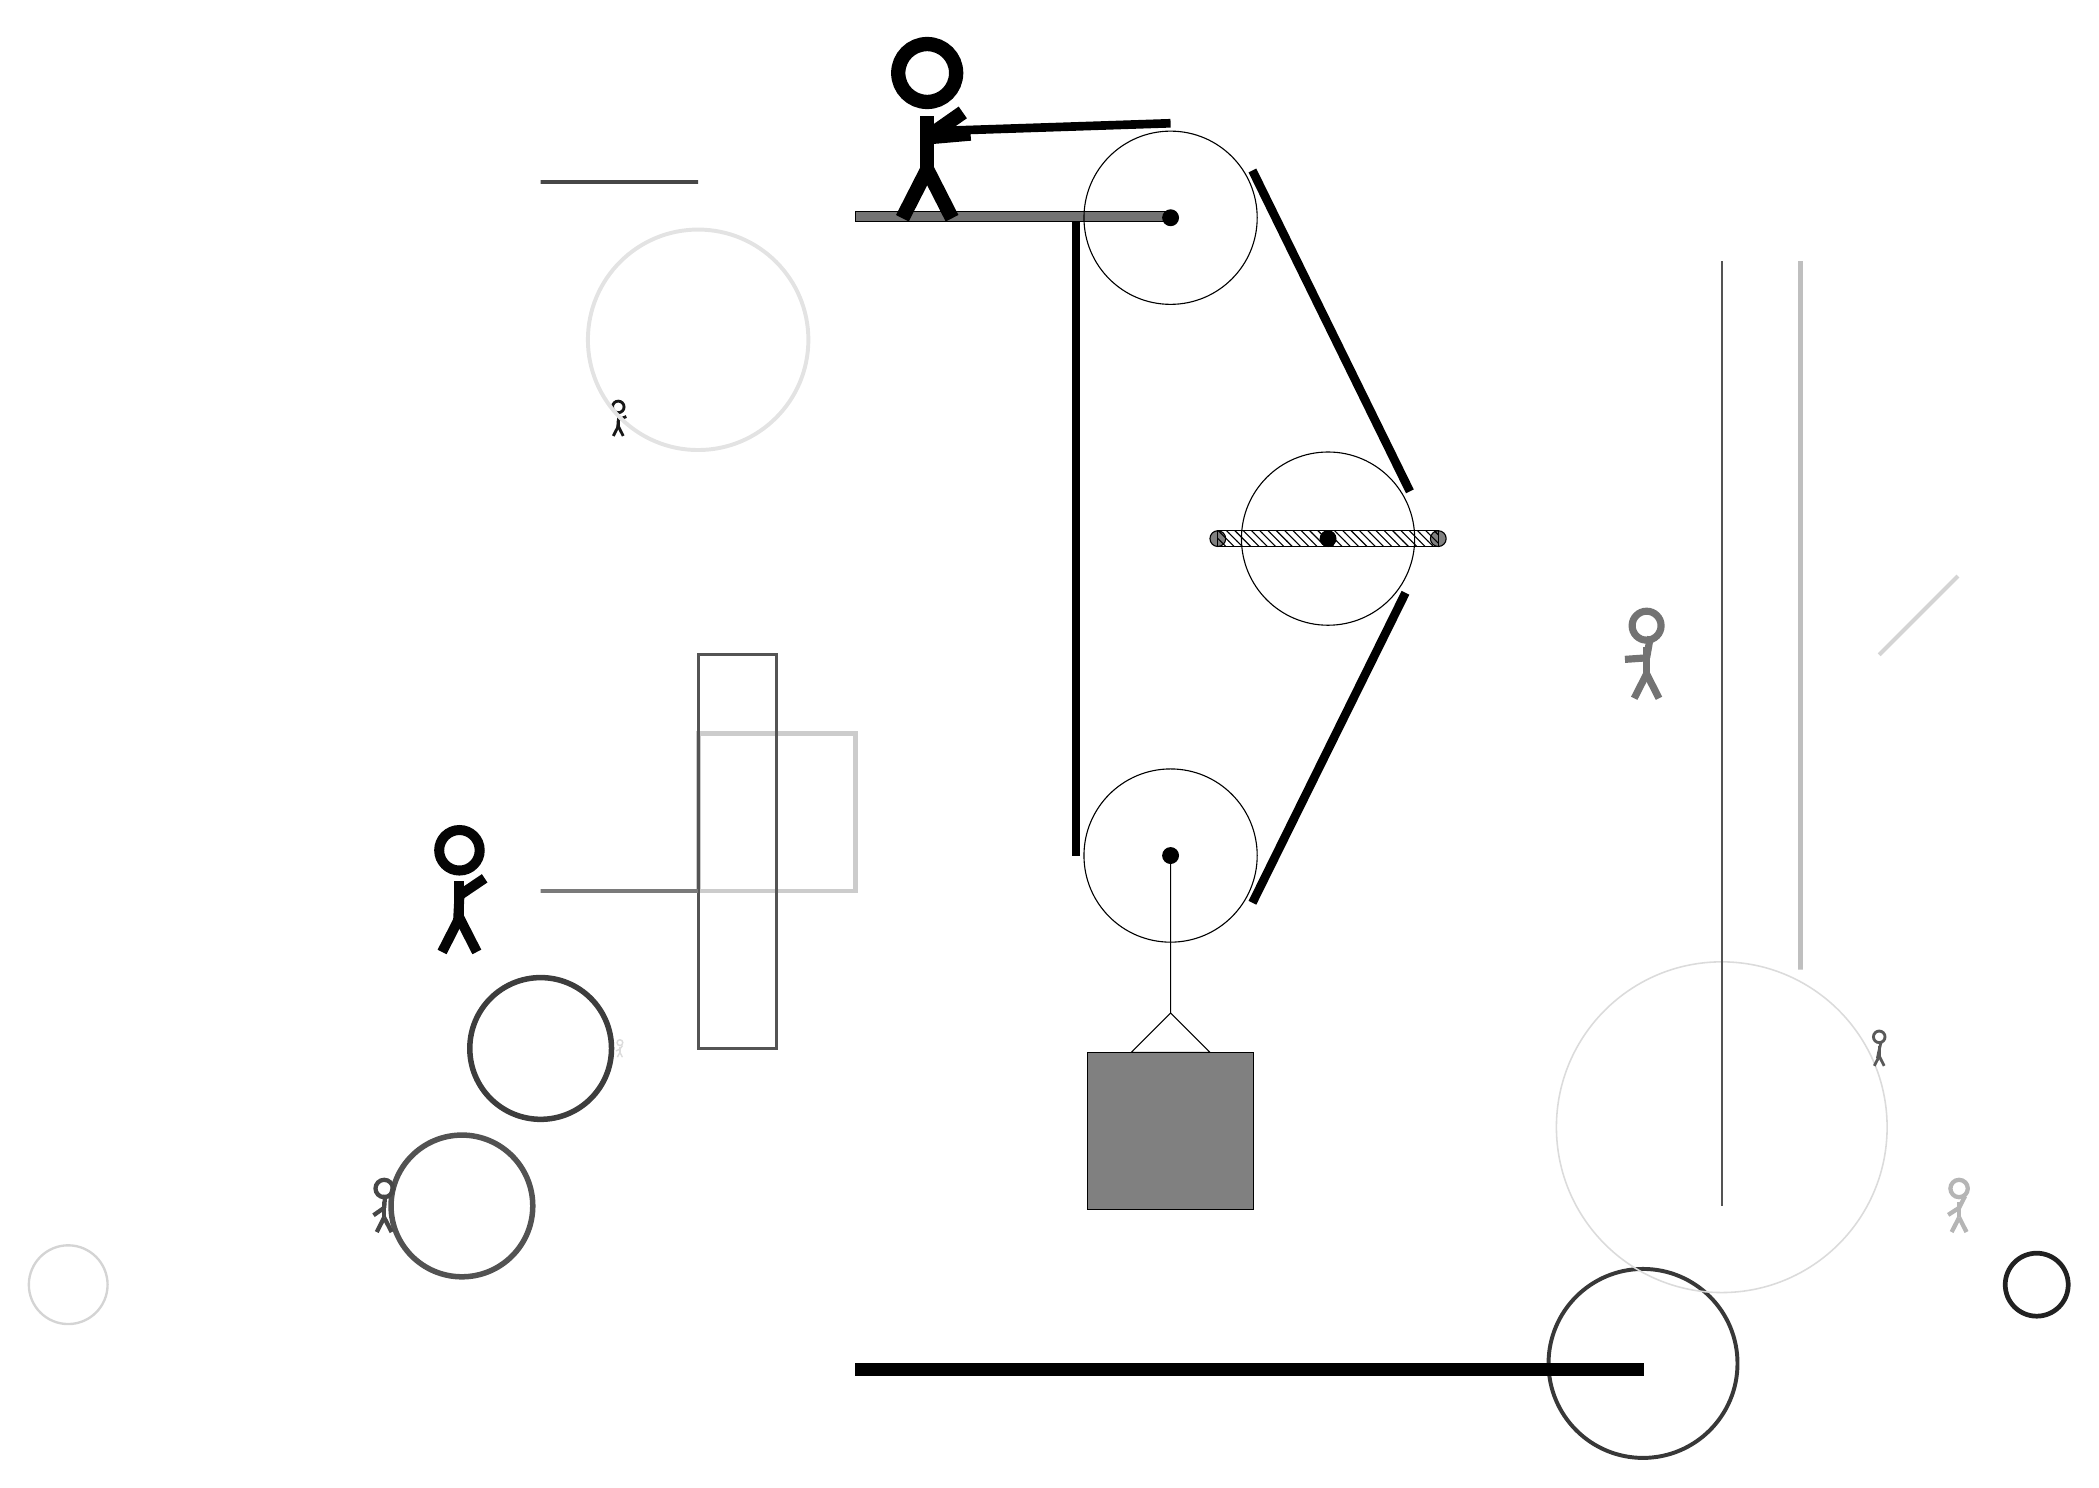
\begin{tikzpicture}
			%%%%% START %%%%%
			
			\draw[fill=black!55] (-2, 11.5) rectangle (2, 11.625);
			
			\draw (2, 3.45) circle (1.1);
			\draw[fill=black] (2, 3.45) circle (0.1);
			
			\draw [line width=0.5mm, color=black!78](8, -3) circle (1.2);
			
			\draw [line width=0.7mm, color=black!68](-7, -1) circle (0.9);
			\draw[line width=0.5mm, color=black!17](11, 6) -- (12, 7);
			\node[line width=0.2mm, color=black!14] at (-5, 1) {\Strichmaxerl[1][25][54]};
			
			\draw [line width=0.3mm, color=black!17](-12, -2) circle (0.5);
			\draw [line width=0.6mm, color=black!87](13, -2) circle (0.4);
			
			\draw [line width=0.2mm, color=black!14](9, 0) circle (2.1);
			
			\draw[line width=0.6mm, color=black!20] (-2, 3) rectangle (-4, 5);
			\node[line width=0.5mm, color=black!29] at (12, -1) {\Strichmaxerl[3][33][63]};
			\node[line width=0.6mm, color=black!91] at (-5, 9) {\Strichmaxerl[2][86][22]};
			
			\node[line width=0.5mm, color=black!98] at (-7, 3) {\Strichmaxerl[7][87][34]};
			\draw[line width=0.2mm, color=black!67] (9, 11) rectangle (9, -1);
			\draw [line width=0.7mm, color=black!76](-6, 1) circle (0.9);
			
			\node[line width=0.5mm, color=black!65] at (11, 1) {\Strichmaxerl[2][78][77]};
			\node[line width=0.4mm, color=black!72] at (-8, -1) {\Strichmaxerl[3][35][86]};
			\draw[line width=0.4mm, color=black!67] (-3, 6) rectangle (-4, 1);
			
			\draw [line width=0.5mm, color=black!11](-4, 10) circle (1.4);
			
			\draw[line width=0.5mm, color=black!72] (-4, 12) rectangle (-6, 12);
			\node[line width=0.3mm, color=black!55] at (8, 6) {\Strichmaxerl[5][4][80]};
			\draw[line width=0.4mm, color=black!52] (-4, 3) rectangle (-6, 3);
			\draw[line width=0.6mm, color=black!25] (10, 11) rectangle (10, 2);
			
			\draw (2, 11.55) circle (1.1);
			\draw[fill=black] (2, 11.55) circle (0.1);
			
			\draw[fill=white](4, 7.475) circle (1.1);
			\draw[fill=black] (4, 7.475) circle (0.1);
			\draw[fill=black!50] (2.6, 7.475) circle (0.1);
			\draw[fill=black!50] (5.4, 7.475) circle (0.1);
			\draw[pattern=north west lines, pattern color=black] (2.6, 7.575) rectangle (5.4, 7.375);
			
			\draw (2, 3.45) -- (2, 1.45) -- (1.5, 0.95) -- (2.5, 0.95) -- (2, 1.45);
			\draw[fill=black!50] (0.95, 0.95) rectangle (3.05, -1.05);
			
			\draw[line width=1.1mm] (0.8, 11.5) -- (0.8, 3.45);
			\centerarc[line width=1.1mm](2, 3.45)(180:330:1.2000000000000002);
			\draw[line width=1.1mm](3.0392, 2.85) -- (4.983, 6.7867);
			\centerarc[line width=1.1mm](4, 7.475)(390:325:1.2000000000000002);
			\draw[line width=1.1mm](5.0392, 8.075) -- (3.0392, 12.15);
			\centerarc[line width=1.1mm](2, 11.55)(30:90:1.2000000000000002);
			\draw[line width=1.1mm](2, 12.75) -- (-1, 12.65);
			
			\node at (-1, 12.65) {\Strichmaxerl[10][-175][35]};
			
			\draw[fill=black] (-2, -3) rectangle (8, -3.15);
			
			%%%%% END %%%%%
		\end{tikzpicture}
	\end{figure}	
\end{document}